\newpage
\section{Oppbygging av programmet}
\thispagestyle{fancy}

\subsection{Programmeringsmetode}
For å sette saman alle funksjonsblokkene vi hadde programmert i \gls{ST}, valde vi å nytte \gls{Codesys} ``Continuous Function Chart'' (\gls{CFC}).
\gls{CFC} er eit grafisk programmeringsspråk som nyttar symbol og koplingar for å gjere programmet meir visuelt.

Alle samankoplingar av blokker valde vi å gjere i \gls{CFC}. Ved å nytte ein grafisk metode sikra vi oss god lesbarheit og
visuell forståelse av programmet. 

Alle inngangar og utgangar er leselege og enkle og forstå. \gls{CFC} i lag med god dokumentasjon vil kunne gi personar utan programmeringsbakgrunn
god forståelse av korleis programmet er oppbygd, utan å måtte lese kodelinjer.
\gls{CFC} gir eit godt grunnlag for feilsøking og analyse, dette bygger vidare på filosofien med eit enkelt og fleksibelt program.

Dersom antall koplingar og linjer gjorde programmet vanskeleg å lese var det også
mogleg å opprette ``source'' og ``links'' som oppretta ein trådlaus forbindelse gjennom ein unik ID.

\begin{figure}[htbp]
    \centering
    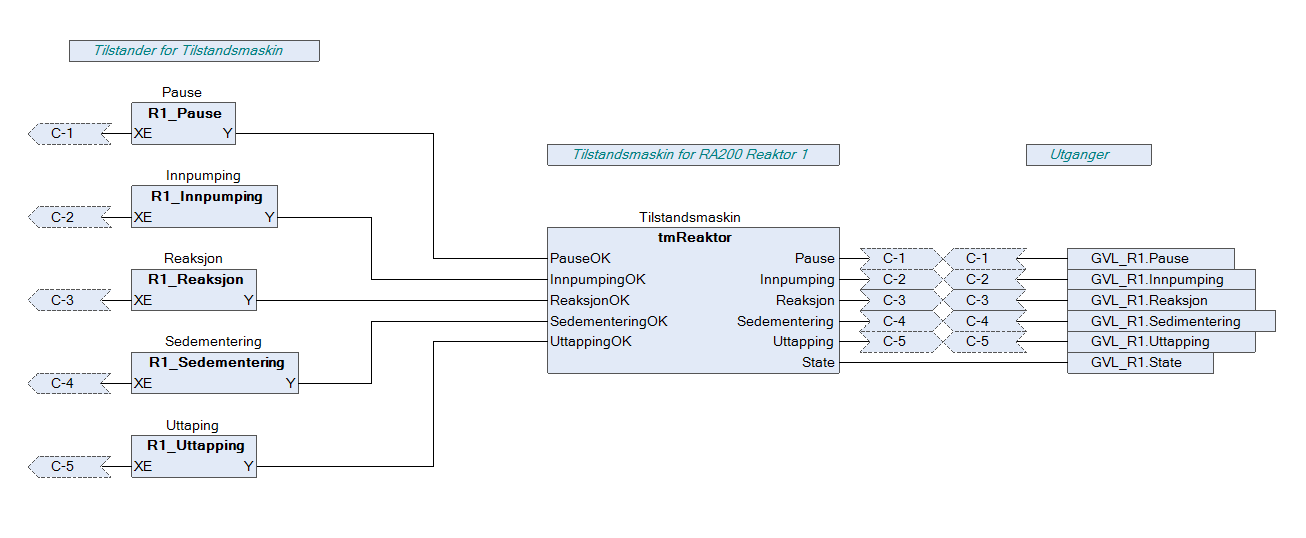
\includegraphics[width=1\textwidth]{Bilder/ReaktorPRG.png}
    \caption{Eksempel \gls{CFC} - Styring reaktor 1}\label{fig:CFCReaktor}
\end{figure}

\newpage

\subsection{Hovuddel}

Programmet er delt opp i tre hovuddelar, ei tilstandsmaskin for kvar reaktor og ein del for samling av felles reaktorfunksjonar.
Alle delane blir utført kvar \gls{PLS} syklus. 
Tilstandsmaskina har det overordna ansvaret og passar på kva tilstandslogikkblokk som nyttast.

Fellesfunksjonar er ei samling av funksjonsblokker og utrekningar som er felles for reaktorane, og er uavhengig av tilstandsmaskinene.
Driftsovervaking er ein sentral del av fellesfunksjonar, der gangtider og mengde prosessert vatn er døme utførte berekningar.

I nokre tilfelle, som ved rullering av sivbed, var vi avhengig at begge tilstandsmaskinene hadde same informasjon.
Dette løyste vi ved å lage ei funksjonsblokk ``fbSivbedRotation'', i felles funksjonar, som hentar inn og behandlar antall slamuttak for å rotere sivbed når ei gitt grense er nådd.
Denne informasjonen blir deretter sendt til kvar tilstandsmaskin som sørger for at begge reaktorane har same aktive sivbed.

\begin{figure}[htbp]
    \centering
    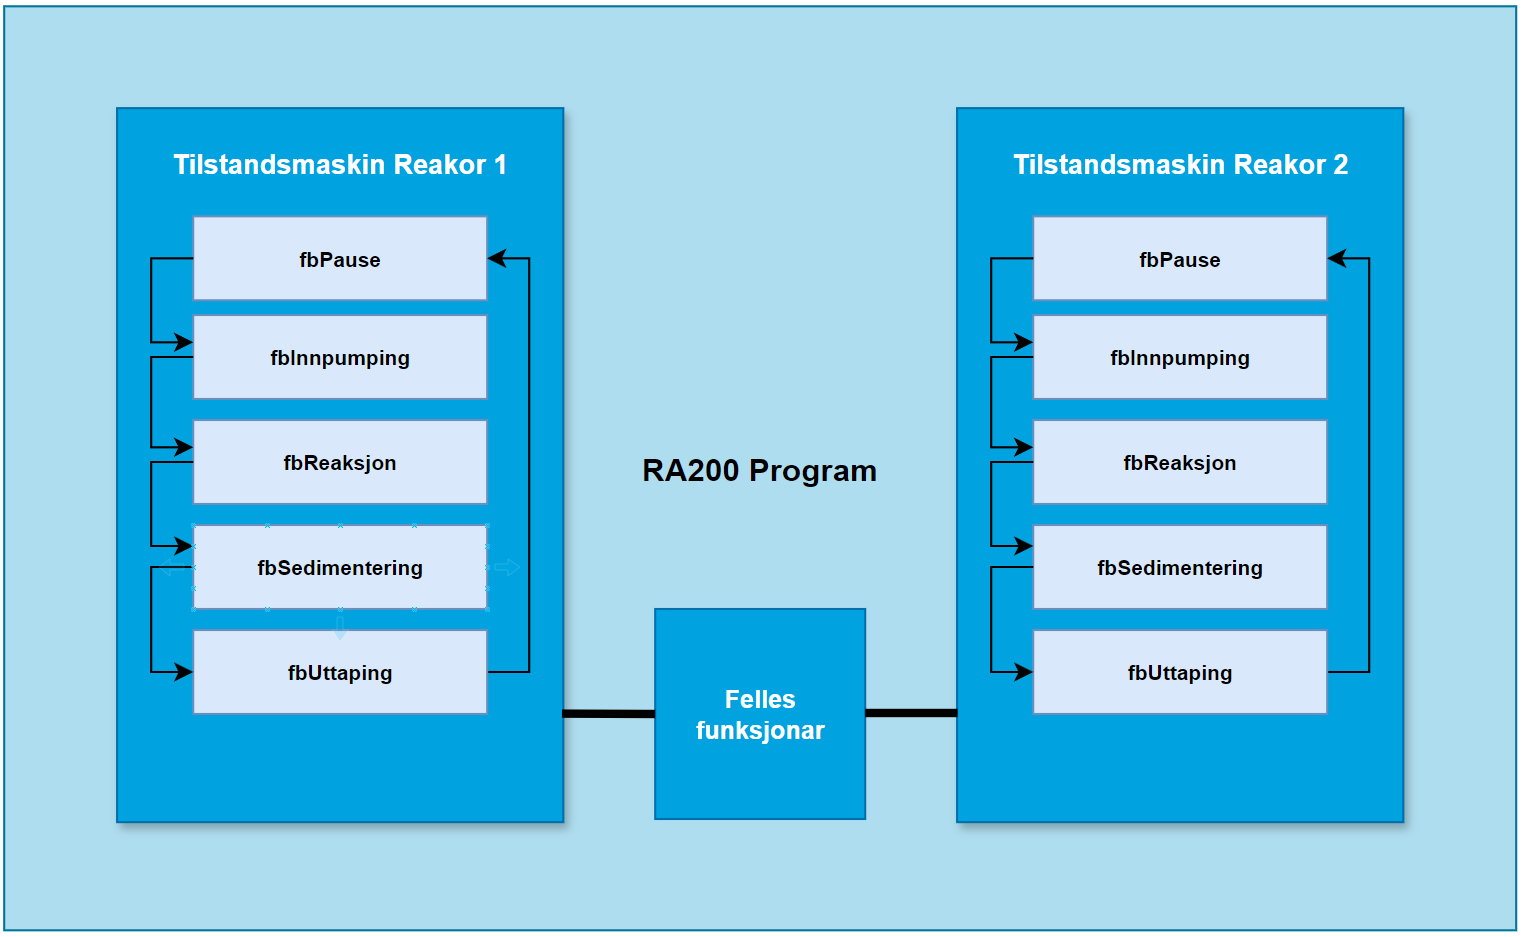
\includegraphics[width=1\textwidth]{Figurar/Oppbygging_Program.png}
    \caption{Illustrasjon oppbygging program}\label{fig:OppbyggingProgram}
\end{figure}

\newpage

\subsection{Styring tilstandslogikk}

Som tidlegare skildra er det tilstandslogikken som samarbeider med \gls{IEC}-blokkene. Dette samarbeidet valde vi også å gjere i eit
\gls{CFC} vindauge som gjorde kall og koplingar meir visuelt. \gls{CFC} vindauget fikk namn etter kva sekvens i \gls{SBR}-prosessen
den hadde ansvar for å styre. 

Oppbygginga av desse sekvensstyringane er gjort med inngangsblokker (\gls{MA} og \gls{MB}) øvst og utgangsblokker (\gls{SBE} og \gls{SBV}) i botn.
Mellom desse kjem tilstandslogikkblokka som inneheld styringslogikk.

\begin{figure}[htbp]
    \centering
    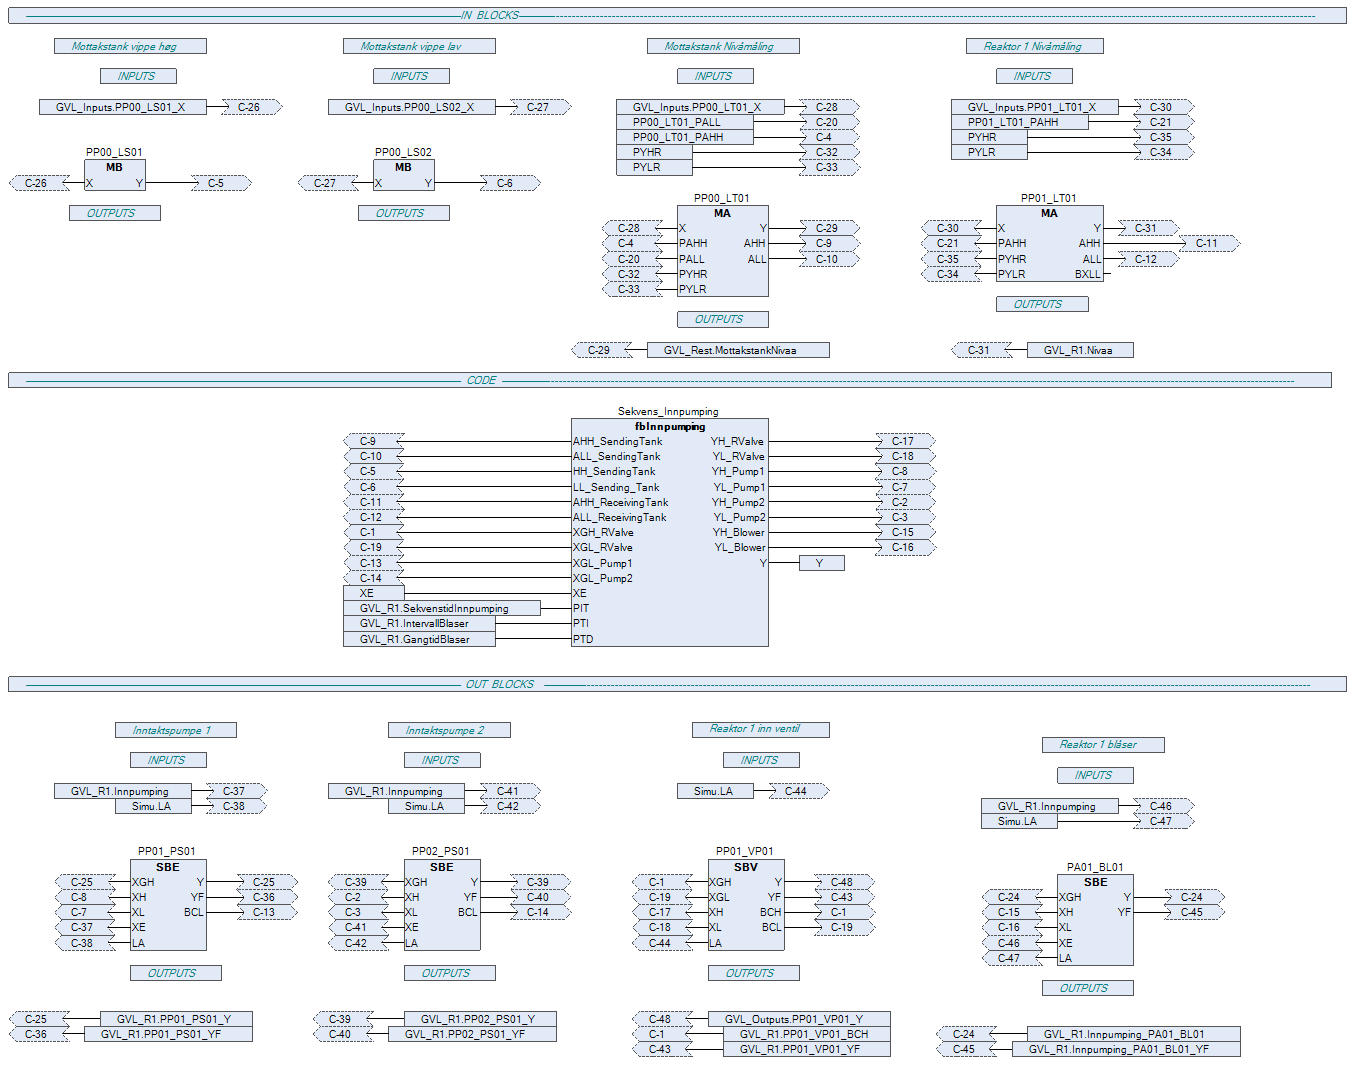
\includegraphics[width=1\textwidth]{Bilder/Heile_innpump.png}
    \caption{Eksempel \gls{CFC} - styring innpumping}\label{fig:CFCInnpumping}
\end{figure}

I denne figuren er ekstra inngangar, parameterinngangar og utgangar fjerna for å betre kunne visualisere koplingane og samarbeidet mellom
\gls{IEC}-blokkene og tilstandslogikk.

\newpage

